% Chapter Template

\chapter{Related work} % Main chapter title

\label{ch:rw} % Change X to a consecutive number; for referencing this chapter elsewhere, use \ref{ChapterX}

\lhead{Chapter \ref{ch:rw}. \emph{Related work}} % Change X to a consecutive number; this is for the header on each page - perhaps a shortened title

%----------------------------------------------------------------------------------------
%	INTRO TEXT
%----------------------------------------------------------------------------------------
The goal of this thesis, to design and implement a \textbf{learning-capable} dialogue system, combines different disciplines within the fields of Artificial Intelligence and Linguistics. This chapter reviews the most relevant work that has been previously done, and that contributed to the realization of this project.

%----------------------------------------------------------------------------------------
%	SENTENCE SIMILARITY
%----------------------------------------------------------------------------------------

\section{Sentence similarity}
As it has been mentioned in the previous chapter, the core task of the system is to associate an unknown sentence to its correct meaning, where each meaning is defined by a set of sentences realizing it. Therefore, one of the constituent capabilities that the system must implement is the ability to tell whether two sentences \textbf{share the same meaning} or not.

The problem of scoring the similarity between two sentences is not new in the literature, and a number of different approaches already exist to tackle it. \cite{Achananuparp:2008:ESS:1430555.1430594} suggest to classify the existing measures in \textbf{three categories}: word overlap measures, TF-IDF measures and Linguistic measures. \textbf{Word overlap} scores are computed taking into account only the number of words that are shared between the two input sentences; a basic measure of this kind is the Jaccard coefficient, which is defined as the size of the intersection of the words in the two sentences compared to the size of the union of the words in the two sentences. \cite{Banerjee03extendedgloss} extended the concept to include a special treatment of phrasal $n$-word overlaps, motivated by the fact that they are much rarer than single word ones. \textbf{TF-IDF} measures are based on term frequency-inverse document frequency, hence the name. Those are common measures to express the importance of a term of a document in an  indicized corpus; respectively, they represent the frequency of the term in the document, and the frequency of the term across all documents. TF-IDF can be used to score the similarity between two sentences, for instance, computing the cosine similarity in a vector-space approach. Lastly, \textbf{linguistic} measures are meant to exploit, intuitively, the linguistic information contained in the input sentences. Such information consists of semantic relations between words, and the syntactic structure that connects them. % Various methods exist to ...

The way sentences are compared in \pname takes into account the aspects of all these three types of measures, which are combined together in a feature-oriented fashion; the specific algorithm for sentence comparison is described in Chapter \ref{ch:M2}.

%----------------------------------------------------------------------------------------
%	IBM WATSON
%----------------------------------------------------------------------------------------

\section{Machine Learning for Language Processing}
The task of labeling an unknown sentence with its correct meaning can be easily expressed in terms of Machine Learning. In fact, it is a standard supervised \textbf{classification problem} to learn a class' model from examples, and later use that model to label new data points. In this view, a data point is a natural language sentence, and a label is its meaning. 

\subsection{Computational Linguistics}
Another source of inspiration for this work is represented by \textbf{statistic}, corpus-based methods in Computational Linguistics; a significant example comes from The IBM models for Statistical \textbf{Machine Translation} \citep{Brown:1993:MSM:972470.972474}, that first introduced the idea of feeding statistically intensive \textbf{Machine Learning} algorithms with big data from corpora, which nowadays is the dominant paradigm in MT; insightful is also the work on Data Oriented Parsing, and particularly the U-DOP model for \textbf{Unsupervised Language Learning} \citep{Bod:2006:UPU:1596276.1596293}, which core idea is to initially assume all the possible syntax trees for a set of sentences as equally possible, and then use all the possible sub-trees of them to compute the most probable parse trees, letting the structure of the language emerge from the data.

This work in Computational Linguistics is well reflected in our project, as a strong part of it consists of finding \textbf{alignments} of strings sharing similar meanings. We will see (Chapters \ref{ch:arch} and \ref{ch:M2}) that the computation of these alignments happens in a similar setting as in corpus-based Machine Translation: every alignment is initially considered plausible\footnote{It is worth to note that, where in classic Machine Translation every alignment is initially considered possible with equal probability, here we use some heuristics to provide a clever initialization, in order to cope with the limited amount of training data we have.}, but recurrent ones are reinforced more often, and will thus achieve better and better scores as the model is trained with more examples Also, the same procedure that computes the alignments is used to let \textbf{syntactic structures} emerge from training data, and from processing new input sentences.

\subsection{IBM Watson}
Particularly inspiring for the development of this thesis was the work done by IBM on Watson. \textbf{IBM Watson} is a question answering computer system that applies advanced Artificial Intelligence techniques to the field of open domain question answering \citep{Ferrucci:2011:IW:2024723.2019525}. That is, a software capable of crawling a database of knowledge looking for an answer to any specific English question given as input; along with the answer, the system outputs also a confidence value, that accurately reflects the probability of the answer being correct. Watson was in the headlines in 2011 for competing in the popular American quiz show \textit{Jeopardy!}, defeating former winners  Brad Rutter and Ken Jennings, and thus winning the \$1 million first prize.

What is interesting about Watson, respect to our work, is the feature-based approach to \textbf{evidence scoring} that is used to select the correct answers. Figure \ref{ch:rw:ml:watson} \citep{journals/aim/FerrucciBCFGKLMNPSW10} shows a bird-eye view of the whole Watson architecture; the part of this process that is especially interesting for us is the \textit{Hypothesis and evidence scoring}: at that point, the system receives a set of candidate answers for the input question; each of this answers will be run through a series of procedures whose purpose is to find evidence supporting that answer. Most of these procedures are not particularly sophisticate, in fact the clever part of the algorithm is to combine a \textbf{high number of features} to obtain an accurate final score value. This is done by training Watson's hypermodel with data from previous \textit{Jeopardy!} games; the hypermodel consists of a set of weights, that are then used to produce the optimal linear combination of the features.

Even though this latter meta-learning aspect is not implemented in our work, we will find a similar feature-based scoring approach in the core matching algorithm of the Language Unit, discussed in detail in Chapter \ref{ch:M2}.

\begin{figure}
	\centering
	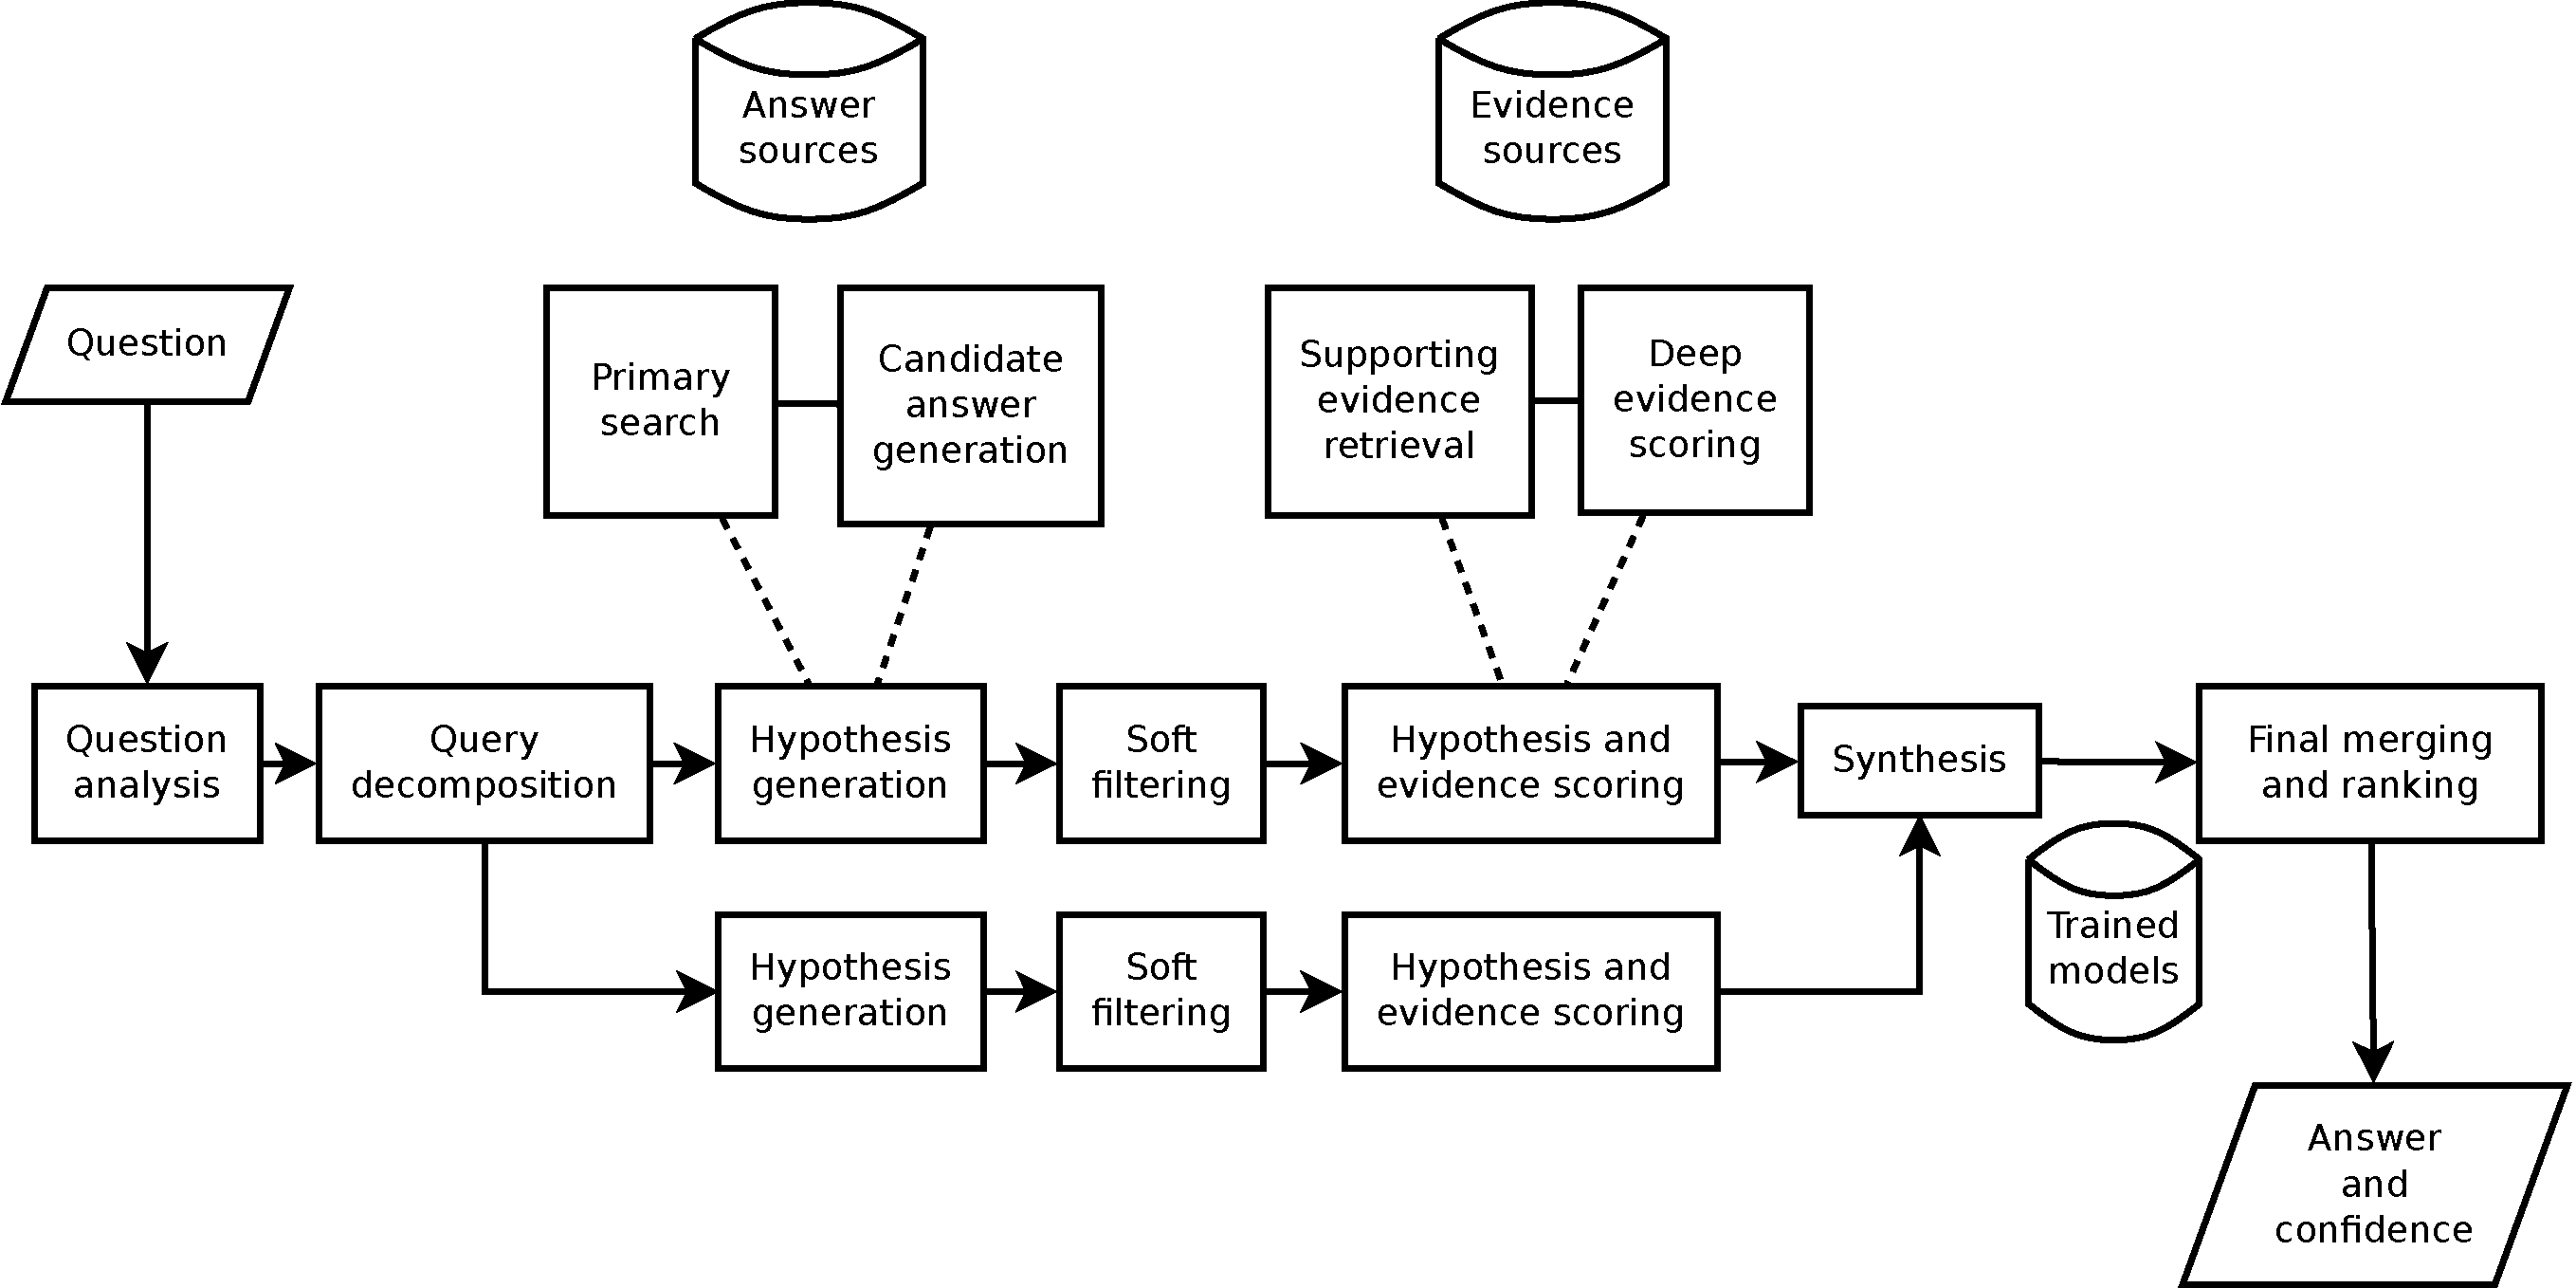
\includegraphics[width=12cm]{Pictures/DeepQA.pdf}
	\caption{Watson's high level architecture}
	\label{ch:rw:ml:watson}
\end{figure}



%----------------------------------------------------------------------------------------
%	DIALOGUE SYSTEMS
%----------------------------------------------------------------------------------------

\section{Dialogue Systems}

Research on dialogue systems has been carried on since the \textbf{early days} of Artificial Intelligence. A milestone in the early work on this field is ELIZA \citep{Weizenbaum:1966:ECP:365153.365168}, which provides the user with a basic human-like interaction based on pattern matching; another example is the SHRDLU system \citep{winograd1971procedure}, which interfaces the user with a simple spatial domain by listening to the user's utterances (e.g.\ ``Would you please put the green pyramid in the box?"), and performing actions accordingly in the domain, resolving, if necessary, ambiguous or implicit references to the entities in it.

According to \cite{Jokinen2009}, modern dialogue systems can be divided in \textbf{two main types}: task-oriented and nontask-oriented. Intuitively, systems in the first category are meant to deal with a specific task such as making a hotel booking, or booking a plane ticket; an example in this category is the MIT Mercury system, a vocal interface to a flight database \citep{Seneff:2000:DMM:1605285.1605288}. On the other hand, nontask-oriented systems are meant to engage in conversations without a specific purpose to fulfill, but the one of delivering a realistic simulation; ELIZA itself is an example of nontask-oriented dialogue system.

Task-oriented systems can be very simple, as simple and well-formalized the task is;  many applications, such as travel service or call routing, can be successfully solved by \textbf{slot-based} systems: each step of the conversation requires some pieces of information, modeled as slots, to be filled in by the user (departure city, arrival city, date, and so on); given the slots to be filled, the dialogue task can be solved with a formal grammar of interaction. As the complexity increases, more phenomena of human interaction have to be modeled, such as turn-taking, multimodality or grounding
%\ignore{CITE RAQUEL'S CHAPTER}
, as well as semantic structures such as quantification and negation; slot-based systems are not sufficient to model these scenarios \citep{Gabsdil03clarificationin}, that require more advanced frameworks such a the Information State Update (ISU) one \citep{TraumLarsson03p325}.

\subsection{Information State Update Dialogue Management}

\ldots